The controller was designed using a parallel \gls{pd} structure. The initial
gains were obtained using the Ziegler--Nichols tuning method based on
\Eqref{planta-sensor-1-zn} and were subsequently refined using the \gls{rmse},
defined by \Eqref{rmse}, as the performance criterion.

\begin{equation}
\eqlabel{rmse}
\mathrm{RMSE} = \sqrt{\frac{1}{N}\sum_{k=1}^{N}{\left( r[k] - y[k] \right)}^{2}}
\end{equation}

The resulting \gls{pd} controller is given by \Eqref{controlador-pd-paralelo}.

\begin{equation}
\eqlabel{controlador-pd-paralelo}
C_{\mathrm{pd}}(s) = 13.472 + \frac{601.4s}{s+100}
\end{equation}

Although the \gls{pd} controller provided satisfactory dynamic performance, it
still exhibited a noticeable \gls{ess} when tracking the reference signal.

To reduce this error, a \gls{ff} action was added based on an inverse plant
model combined with a filter that specifies the desired closed-loop
dynamics~\cite{astrom2021feedback,seborg2016process}.
This control strategy uses the process model to anticipate the control action
required for reference tracking~\cite{astrom2021feedback}.

In this paper, the \gls{ff} controller was implemented using the inverse model
of the plant described by \Eqref{planta-sensor-1-zn}, operating in parallel with
the \gls{pd} controller, together with a low-pass filter to ensure causality.
The resulting feed-forward controller is given by \Eqref{controlador-ff}:

\begin{equation}
\eqlabel{controlador-ff}
C_{\mathrm{ff}} = \frac{188.0271s + 1}{6.075 s + 0.92}
\end{equation}

\Figref{bloco-controlador} shows the complete control structure. The \gls{ff}
controller acts directly on the reference signal, while the \gls{pd} controller
compensates for the tracking error through system feedback.

\begin{figure}[H]
\centering
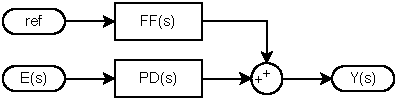
\includegraphics[width=0.9\linewidth]{images/Bloco Controlador.pdf}
\caption{Proposed control structure composed of a \gls{ff} action applied to the
reference signal and a \gls{pd} action based on system feedback.}
\figlabel{bloco-controlador}
\end{figure}

The controller was discretized using the Tustin method, applied to both the
\gls{pd} and \gls{ff} controllers. In this method, the continuous-time operator
$s$ is approximated by the bilinear transformation given in \Eqref{tustin}:

\begin{equation}
\eqlabel{tustin}
s \approx \frac{2}{T_s}\frac{z-1}{z+1}
\end{equation}

Where $T_s$ is the sampling period, defined as $T_s = \SI{15}{\second}$. The
plant model was discretized using \gls{zoh}, resulting in \Eqref{planta-gz-zoh}.

\begin{equation}
\eqlabel{planta-gz-zoh}
G(z) = z^{-1} \cdot \frac{0.0413z + 0.0293}{z - 0.9233}
\end{equation}
